\documentclass[12pt, twoside]{article}
\usepackage[letterpaper, margin=1in, headsep=0.5in]{geometry}
\usepackage[english]{babel}
\usepackage[utf8]{inputenc}
\usepackage{amsmath}
\usepackage{amsfonts}
\usepackage{amssymb}
\usepackage{tikz}
\usetikzlibrary{quotes, angles}
\usepackage{graphicx}
\usepackage{enumitem}
\usepackage{multicol}

\newif\ifmeta
\metatrue %print standards and topics tags

\title{Regents Geometry}
\author{Chris Huson}
\date{September 2020}

\usepackage{fancyhdr}
\pagestyle{fancy}
\fancyhf{}
\renewcommand{\headrulewidth}{0pt} % disable the underline of the header
\raggedbottom


\fancyhead[LE]{\thepage}
\fancyhead[RO]{\thepage \\ Name: \hspace{4cm} \,\\}
\fancyhead[LO]{BECA / Dr. Huson / Geometry \\* 1-7 Angle measures}

\begin{document}

\subsubsection*{I can add the measures of angles}
\begin{enumerate}
  \item Do Now: Given $M$ is the midpoint of $\overline{AB}$, $AM=5x+2$, $MB=20$.
  \begin{enumerate}
    \item Mark the diagram with the values and tick marks
    \item Write an equation and solve for $x$
    \item Check your result
  \end{enumerate}
    \begin{center}
      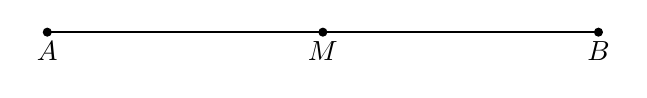
\begin{tikzpicture}
        \draw [fill] (0,0) circle [radius=0.05] node[below]{$A$};
        \draw [-, thick] (0,0)--(7,0);
        \draw [fill] (3.5,0) circle [radius=0.05] node[below]{$M$};
        \draw [fill] (7,0) circle [radius=0.05] node[below]{$B$};
        %\node at (1.7,0.5) [above]{$x+2$};
        %\node at (5.2,0.5) [above]{$11$};
        %\draw [<->, dashed] (0,-1)--(7,-1);
        %\node at (3.5,-1) [below]{$20$};
      \end{tikzpicture}
    \end{center} \vspace{2cm}

\item Given a straight line and a ray, making two angles.
  \begin{enumerate}[itemsep=0.5cm]
    \item Write down the names of the two angles using proper notation.
    \item Using a protractor, measure the two angle in degrees.
    \item Do they sum to $180^\circ$?
  \end{enumerate}
  \begin{center}
  \begin{tikzpicture}
    \draw [<->, thick] (-6,0)--(6,0);
    \draw [thick, ->] (0,0)--(60:5);
    \draw [fill] (0,0) circle [radius=0.05] node[below]{$A$};
    \draw [fill] (-4,0) circle [radius=0.05] node[below]{$B$};
    \draw [fill] (4,0) circle [radius=0.05] node[below]{$D$};
    \draw [fill] (60:4) circle [radius=0.05] node[right]{$C$};
  \end{tikzpicture}
  \end{center}

\item For each example, explain the error made drawing $\overrightarrow{JK}$.\\.\\
\vspace{0.5cm}
  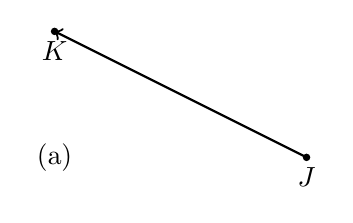
\begin{tikzpicture}[scale=.8]
    \draw  [<-, thick] (0,2)--(4,0);
    \draw [fill] (0,2) circle [radius=0.05] node[below]{$K$};
    \draw [fill] (4,0) circle [radius=0.05] node[below]{$J$};
    \node at (0,0) {(a)};
  \end{tikzpicture}  \hspace{1cm}
  \begin{tikzpicture}[scale=.8]
    \draw  [<-, thick] (-1,2.5)--(4.4,-0.2);
    \draw [fill] (0,2) circle [radius=0.05] node[below]{$K$};
    \draw [fill] (4,0) circle [radius=0.05] node[below left]{$J$};
    \node at (0,0) {(b)};
  \end{tikzpicture} \hspace{1cm}
  \begin{tikzpicture}[scale=.8]
    \draw  [<-, thick] (-1,2.5)--(0,2)--(2,1.1)--(3,0.4)--(4,0);
    \draw [fill] (0,2) circle [radius=0.05] node[below]{$K$};
    \draw [fill] (4,0) circle [radius=0.05] node[below]{$J$};
    \node at (0,0) {(c)};
  \end{tikzpicture}
  \vspace{4cm}
  
\newpage
\item Write down the name of the \emph{three} angles shown in the diagram below and their angle measures, using your protractor.
    \begin{center}
    \begin{tikzpicture}[scale=2]
      \draw [->, thick] (0,0)--(15:4);
      \draw [->, thick] (0,0)--(95:4);
      \draw [->, thick] (0,0)--(130:4);
      \draw [fill] (15:3) circle [radius=0.03] node[below]{$B$};
      \draw [fill] (95:2) circle [radius=0.03] node[right]{$C$};
      \draw [fill] (0,0) circle [radius=0.03] node[left]{$A$};
      \draw [fill] (130:2) circle [radius=0.03] node[left]{$D$};
    \end{tikzpicture}
    \end{center}

\item Given the situation in the diagram, answer each question. Circle True or False.
  \begin{center}
  \begin{tikzpicture}[scale=1, rotate=20]
    \draw [->, thick] (0,0)--(4,3);
    \draw [<->, thick] (-5,.5)--(5,-.5);
    \draw [->, thick] (0,0)--(-1.2,3);
    \draw [fill] (-1,2.5) circle [radius=0.05] node[below left]{$S$};
    \draw [fill] (2.66666,2) circle [radius=0.05] node[above left ]{$T$};
    \draw [fill] (0,0) circle [radius=0.05] node[below]{$P$};
    \draw [fill] (4,-0.4) circle [radius=0.05] node[above]{$U$};
    \draw [fill] (-4,0.4) circle [radius=0.05] node[above]{$R$};
  \end{tikzpicture}
  \end{center}
  \begin{enumerate}
  \item True or False: $\overrightarrow{RP}$ and $\overrightarrow{UP}$ are opposite rays.\bigskip
  \item True or False: $\angle TPR$ is an obtuse angle.\bigskip
  \item True or False: $\angle RPS$ and $\angle SPU$ are supplementary angles.\bigskip
  \item True or False: $\angle RPS$ and $\angle SPT$ are adjacent angles. \bigskip
  \end{enumerate}

\end{enumerate}
\end{document}